\documentclass{article}

\usepackage{fancyhdr}
\usepackage{extramarks}
\usepackage{amsmath}
\usepackage{amsthm}
\usepackage{amsfonts}
\usepackage{tikz}
%\usepackage[plain]{algorithm}
%\usepackage{algpseudocode}
\usepackage{mdframed}
\usepackage{listings}
\usepackage{color}
 
\definecolor{codegreen}{rgb}{0,0.6,0}
\definecolor{codegray}{rgb}{0.5,0.5,0.5}
\definecolor{codepurple}{rgb}{0.58,0,0.82}
\definecolor{backcolour}{rgb}{1,1,1}

\usetikzlibrary{automata,positioning}

%
% Basic Document Settings
%

\topmargin=-0.45in
\evensidemargin=0in
\oddsidemargin=0in
\textwidth=6.5in
\textheight=9.0in
\headsep=0.25in

\linespread{1.1}

\pagestyle{fancy}
\lhead{\hmwkAuthorName}
\chead{\hmwkClass\ (\hmwkClassInstructor\ \hmwkClassTime): \hmwkTitle}
\rhead{\firstxmark}
\lfoot{\lastxmark}
\cfoot{\thepage}

\renewcommand\headrulewidth{0.4pt}
\renewcommand\footrulewidth{0.4pt}

\setlength\parindent{0pt}

%
% Create Problem Sections
%

\newcommand{\enterProblemHeader}[1]{
    \nobreak\extramarks{}{Problem \arabic{#1} continued on next page\ldots}\nobreak{}
    \nobreak\extramarks{Problem \arabic{#1} (continued)}{Problem \arabic{#1} continued on next page\ldots}\nobreak{}
}

\newcommand{\exitProblemHeader}[1]{
    \nobreak\extramarks{Problem \arabic{#1} (continued)}{Problem \arabic{#1} continued on next page\ldots}\nobreak{}
    \stepcounter{#1}
    \nobreak\extramarks{Problem \arabic{#1}}{}\nobreak{}
}

\setcounter{secnumdepth}{0}
\newcounter{partCounter}
\newcounter{homeworkProblemCounter}
\setcounter{homeworkProblemCounter}{1}
\nobreak\extramarks{Problem \arabic{homeworkProblemCounter}}{}\nobreak{}

%
% Homework Problem Environment
%
% This environment takes an optional argument. When given, it will adjust the
% problem counter. This is useful for when the problems given for your
% assignment aren't sequential. See the last 3 problems of this template for an
% example.
%

%augmented matrix not part of original template
\makeatletter
\renewcommand*\env@matrix[1][*\c@MaxMatrixCols c]{%
   \hskip -\arraycolsep
   \let\@ifnextchar\new@ifnextchar
   \array{#1}}
\makeatother

\newenvironment{homeworkProblem}[1][-1]{
    \ifnum#1>0
        \setcounter{homeworkProblemCounter}{#1}
    \fi
    \section{Problem \arabic{homeworkProblemCounter}}
    \setcounter{partCounter}{1}
    \enterProblemHeader{homeworkProblemCounter}
}{
    \exitProblemHeader{homeworkProblemCounter}
}

%
% Homework Details
%   - Title
%   - Due date
%   - Class
%   - Section/Time
%   - Instructor
%   - Author
%

\newcommand{\hmwkTitle}{Homework\ Number\ Two}
\newcommand{\hmwkDueDate}{Febuary 14, 2018}
\newcommand{\hmwkClass}{CS\ 432}
\newcommand{\hmwkClassTime}{}
\newcommand{\hmwkClassInstructor}{Alexander Nwala}
\newcommand{\hmwkAuthorName}{\textbf{Tim Bruce}}

%
% Title Page
%

\title{
    \vspace{2in}
    \textmd{\textbf{\hmwkClass:\ \hmwkTitle}}\\
    \normalsize\vspace{0.1in}\small{Due\ on\ \hmwkDueDate\ at 4:20 PM}\\
    \vspace{0.1in}\large{\textit{\hmwkClassInstructor\ \hmwkClassTime}}
    \vspace{3in}
}

\author{\hmwkAuthorName}
\date{}

\renewcommand{\part}[1]{\textbf{\large Part \Alph{partCounter}}\stepcounter{partCounter}\\}

%
% Various Helper Commands
%

% Useful for algorithms
\newcommand{\alg}[1]{\textsc{\bfseries \footnotesize #1}}

% For derivatives
\newcommand{\deriv}[1]{\frac{\mathrm{d}}{\mathrm{d}x} (#1)}

% For partial derivatives
\newcommand{\pderiv}[2]{\frac{\partial}{\partial #1} (#2)}

% Integral dx
\newcommand{\dx}{\mathrm{d}x}

% Alias for the Solution section header
\newcommand{\solution}{\textbf{\large Solution}}

% Probability commands: Expectation, Variance, Covariance, Bias
\newcommand{\E}{\mathrm{E}}
\newcommand{\Var}{\mathrm{Var}}
\newcommand{\Cov}{\mathrm{Cov}}
\newcommand{\Bias}{\mathrm{Bias}}

\lstdefinestyle{mystyle}{
    backgroundcolor=\color{backcolour},   
    commentstyle=\color{red},
    keywordstyle=\color{orange},
    numberstyle=\tiny\color{codegray},
    stringstyle=\color{codegreen},
    basicstyle=\footnotesize,
    breakatwhitespace=false,         
    breaklines=true,                 
    captionpos=b,                    
    keepspaces=true,                 
    numbers=left,                    
    numbersep=5pt,                  
    showspaces=false,                
    showstringspaces=false,
    showtabs=false,                  
    tabsize=2
}

\lstset{style=mystyle}


\begin{document}

\maketitle
\pagebreak

I would like to begin by pointing out that my comments are poorly formatted in ths LaTeX document. I am working on figuring out what is causing them to be inconsistent.
\begin{homeworkProblem}
Write a Python program that extracts 1000 unique 
(collect more e.g., 1300 just in case) links from
Twitter. Omit links from the Twitter domain (twitter.com).

Also note that you need to verify that the final target URI (i.e.,
the one that responds with a 200) is unique.  You could have many
different shortened URIs for www.cnn.com (t.co, bit.ly, goo.gl,
etc.).

You might want to use the streaming or search feature to find URIs. If
you find something inappropriate for any reason you see fit, just
discard it and get some more links.  We just want 1000 links that
were shared via Twitter.

Hold on to this collection and upload it to github -- we'll use it
later throughout the semester.

\textbf{Solution} \newline
After some deliberation, I decided to go about this problem in a slightly different manner that what may have been expected in order to make it more general-use. I broke the program into four parts.
\begin{enumerate}
	\item Stream Tweets with inputtable keyword for designated amount of time.
	\item Remove the links from the tweets, follow the redirects, and remove duplicates. (This step also sorts them in alphabetical order)
	\item Get the number of mementos for histogram analysis.
	\item Create the histogram.
\end{enumerate}
The nice thing about this method, is that after each step all the data is saved, so if not enough data is collected the first time around, more data can be added.

\part
TThe streaming is done almost identically to the tutorial that was provided.\cite{sentdex} The only part that is heavily modified is the onData function in the listener class which I would like to direct your attenition to.

%BELOW IS HOW TO EMBED CODE
\begin{center}
    Listing 1: onData function in the listener class.
\begin{mdframed}
\lstinputlisting[language=Python]{tweetOnData.py}
\end{mdframed}
\end{center}
Note that the function has been modified to take the string 'data' as a parameter. This string is actually the string output of a JSON file, which is read into the Python json data type, which can be used like a dictionary. Using this method, it can append to this JSON file at the end. \newline

Also at the end of this code is the timer that stops the function if enough time has elapsed. This uses the current time at start and compares it to the time when the function is called. It should be noted that it will collect the first Tweet after the timer has technically expired. \newline

The tweets are finally stored with the following format:

\begin{center}
    Listing 2: JSON Format for Storing Tweets.
\begin{mdframed}
\lstinputlisting{tweetJSONex.JSON}
\end{mdframed}
\end{center}
NOTE: Most tweets with the tag 'nasa' are talking about two things:
\begin{enumerate}
	\item Ariana Grande appears to recently have come out with a song called 'NASA' which people are going nuts about.
	\item The official end of attempts to contact the Opportunity Rover on Mars after an astounding fifteen year mission. RIP OPPY :'(
\end{enumerate}

\part
TTo parse the Tweets, the program removes the 'expanded\_url' tagged data from the JSON code above. The program then uses a method from Assignment 1 to follow the links using the urllib library in Python.\cite{urllib} Python's urllib includes a function 'urllib.geturl()' which gets the url of the website after the link has been followed past all of the redirects it may have. \newline

Next, the program removes all of the duplicates by hashing all of the links.

\begin{center}
    Listing 3: Duplicate Removal Function.
\begin{mdframed}
\lstinputlisting[language=Python]{removeDuplicates.py}
\end{mdframed}
\end{center}

Note that on line 4 the function uses the normal hash function included in Python. In the past, I have found that this function is robust and hastle free, so I elected to use it here. The function saves the link and the number of times the link has appeared in a list in the dictionary. At the end, when all of the links are removed, it sorts the links alphabetically.\newline

Finally, the links are saved in a text file with each link taking up a line.

\begin{center}
    Listing 5: Final Links Listed in Order.
\begin{mdframed}
\lstinputlisting{hashedlinks.txt}
\end{mdframed}
\end{center}
NOTE: I didn't know that people used Apple News at all. I found it interesting when I saw these four links in the maddness that is the hashedlinks.txt file. \newline

This concludes the first problem on the homework assignment, but the program for parts one and two is actually just one big program because I got annoyed with juggling a bunch of .py files. The structure will carry through from this problem.
\end{homeworkProblem}

\begin{homeworkProblem}
Download the TimeMaps for each of the target URIs.  We'll use the ODU 
Memento Aggregator, so for example:

URI-R = http://www.cs.odu.edu/

URI-T = http://memgator.cs.odu.edu/timemap/link/http://www.cs.odu.edu/

or:

URI-T = http://memgator.cs.odu.edu/timemap/json/http://www.cs.odu.edu/

(depending on which format you'd prefer to parse)

Create a histogram of URIs vs. number of Mementos (as computed
from the TimeMaps).  For example, 100 URIs with 0 Mementos, 300
URIs with 1 Memento, 400 URIs with 2 Mementos, etc.  The x-axis
will have the number of mementos, and the y-axis will have the
frequency of occurence.

\textbf{Solution} \newline
\part
IIt was fairly straightforward to get the JSON from the URI menitioned in the question. After that, it was just a matter of reading how many mementos the URI had, and sorting them somehow. \newline

The method for sorting the mementos for the histogram incorporates the use of a dictionary. This dictionary stores the number of mementos a URI has as the key. The data that the key points to is just an integer that is the number of URIs that had that many mementos. \newline

The program then writes the dictionary to the mementos.json file using the json.dump() function. Producing a result something like below.

\begin{center}
    Listing 6: Mementos stored in JSON.
\begin{mdframed}
\lstinputlisting{mementos.json}
\end{mdframed}
\end{center}

\part
AAs you can see above, a lot of numbers of mementos are only had by one page. This means that to create a histogram, we will need to group some of them together. \newline

To create a histogram, I used matplotlib, and made extensive use of matplotlibs documentation.\cite{matplotlib} This made it easy to take a simple list of data and display it as a chart. There is not a huge amount of explanation to go along with this part but I do need to credit Joshua Gahan, because I based the numeric categories of my chart off of the one he posted to the class's slack page.

\begin{center}
    Image 1: Histogram Output From Program.
\end{center}
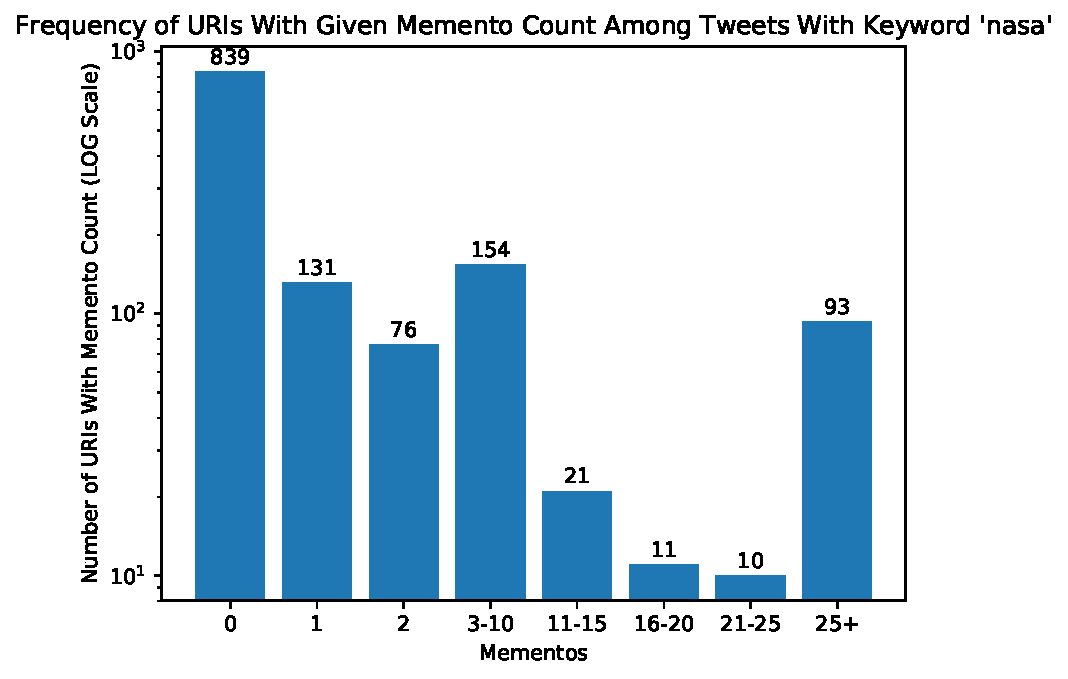
\includegraphics[width=\textwidth]{hist.pdf}
\end{homeworkProblem}

\bibliographystyle{apalike}
\bibliography{bibliography.bib}
\end{document}
